\input{preamble.tex}
\usepackage{lipsum}
\usepackage[toc,page]{appendix}
\usepackage{caption}
\usepackage{hyperref}
\usepackage{svg}
\usepackage{amsmath}
\usepackage{quotes}

\usepackage{listings}

\usepackage{color}
\usepackage{pgfplots}

\usepackage{footnote}
\usepackage{appendix}
\makesavenoteenv{tabular}
\makesavenoteenv{table}

\definecolor{mygreen}{rgb}{0,0.6,0}
\definecolor{mygray}{rgb}{0.5,0.5,0.5}
\definecolor{mymauve}{rgb}{0.58,0,0.82}

\lstset{ %
	basicstyle=\footnotesize,        % the size of the fonts that are used for the code
	breakatwhitespace=false,         % sets if automatic breaks should only happen at whitespace
	breaklines=true,                 % sets automatic line breaking
	captionpos=b,                    % sets the caption-position to bottom
	commentstyle=\color{mygreen},    % comment style
	deletekeywords={...},            % if you want to delete keywords from the given language
	escapeinside={\%*}{*)},          % if you want to add LaTeX within your code
	extendedchars=true,              % lets you use non-ASCII characters; for 8-bits encodings only, does not work with UTF-8
	frame=single,	                   % adds a frame around the code
	keepspaces=true,                 % keeps spaces in text, useful for keeping indentation of code (possibly needs columns=flexible)
	keywordstyle=\color{blue},       % keyword style
	language=Java,                 % the language of the code
	morekeywords={*,...},            % if you want to add more keywords to the set
	numbers=left,                    % where to put the line-numbers; possible values are (none, left, right)
	numbersep=5pt,                   % how far the line-numbers are from the code
	numberstyle=\tiny\color{mygray}, % the style that is used for the line-numbers
	rulecolor=\color{black},         % if not set, the frame-color may be changed on line-breaks within not-black text (e.g. comments (green here))
	showspaces=false,                % show spaces everywhere adding particular underscores; it overrides 'showstringspaces'
	showstringspaces=false,          % underline spaces within strings only
	showtabs=false,                  % show tabs within strings adding particular underscores
	stepnumber=2,                    % the step between two line-numbers. If it's 1, each line will be numbered
	stringstyle=\color{mymauve},     % string literal style
	tabsize=2,	                   % sets default tabsize to 2 spaces \lstinputlisting; also try caption instead of title
}

\begin{document}

\frontmatter

\input{template/colophon}
\input{\mytitlepage}
\input{template/declaration_TU_Graz}
%\cleardoublepage

\tableofcontents

%\chapter{Abstract and Exposeé}

 There are many many different approaches to achieve good software design, however often it is not clear whether the benefits of the best practices overweight the additional effort of implementing them. Little research is done on comparisons between the designs in terms of efficiency and programming effort. Many books do show sample code of their proposed designs, however they do not cover how the code would look like if implemented in a more straight-forward and monolithic way.

This bachelor's thesis tries to cover this topic by implementing the same application two times: as a monolithic program and as a program that pays attention to the information provided about software design and architecture. In the first step, the program will use only one data source and one graphical interface (GUI). In the second step in each program another data source and GUI was added. 

The sourcecode will be available on Github \footnote{\href{https://github.com/Vallant/design-patterns-study.git}{https://github.com/Vallant/design-patterns-study.git}} under GPLv3 \footnote{\href{https://www.gnu.org/licenses/gpl-3.0.de.html}{https://www.gnu.org/licenses/gpl-3.0.de.html}}. The application will be written in Java using Swing as a front-end and PostgreSQL as database. In phase two JavaFX should be supported as a front-end, XML should be supported as a database. The user will be able to choose between all options using parameters when starting the application.

%\begin{table}
\begin{tabular}{|c|l|} \hline
07.04.2017 & Requirements, Complexity and Basic Design of Application \\ \hline
05.05.2017 & Implementation of Best-Practice Approach Phase 1 \\ \hline
26.05.2017 & Implementation of Monolithic Approach Phase 1 \\ \hline
02.06.2017 & Summary of Findings Phase 1 \\ \hline
23.06.2017 & Implementation of Best-Practice Approach Phase 2 \\ \hline
14.07.2017 & Implementation of Monolithic Approach Phase 2 \\ \hline
21.07.2017 & Summary of Findings Phase 2 \\ \hline
28.07.2016 & Thesis finished \\ \hline
\end{tabular}

\caption{Basic Timetable for Bachelor's thesis}
\end{table}



%\input{content/acknowledgements.tex}

\mainmatter

\chapter{Introduction}

The topic of design patterns and architectural styles are vital to the subject of software development. They empower inexperienced programmers to write maintainable applications and provide guidelines that may be adopted but are implemented in each application in one way or another. 

Many books are available on the topic of software design and architectural styles, on how to write maintainable and extensible applications. The books are written by software engineers with many years of experience , like Martin Fowler with his book \emph{Patterns of Enterprise Application Architecture} \footnote{IBAN: 978-0321127426}, Robert C. Martin with \emph{Agile Software Development. Principles, Patterns, and Practices} \footnote{IBAN: 978-0135974445} or \emph{Design Patterns. Elements of Reusable Object-Oriented Software} by John Vlissides, Richard Helm, Ralph Johnson and Erich Gamma \footnote{IBAN: 978-0201633610}. 

The same topics are to a certain degree taught at universities however they all lack one substantial flaw: While they propose some pattern, explain when it is applying and how to implement it, they do not provide any evidence that when using the pattern in a real-world application there is an advantage to gain.  Many patterns claim that they improve the extensibility and increase the decoupling of code however in most of the example code only the basic implementation is showed. The impact on the code when a extension is actually implemented is not being shown by the books which leaves the reader to believe the promises made by the author. 


While the patterns are in extensive use and thus have empirically proven themselves useful,the scientific research on this topic is far from being exhaustive. A study of 2008 was published at IEEE that tried to cover the effect of using design patterns in software development. This study came to the result that while the implementation of best practice methods in many cases enhanced some quality aspects while at the same time performing worse in other factors. It concluded that the use of patterns should be considered carefully as they lead to a certain trade-off.

Another study published covering a similar subject came to different results, concluding that the use of established design patterns in most of the cases led to a significant improvement of code quality, contradicting the previous study. \href{http://ieeexplore.ieee.org/abstract/document/4493325/?reload=true}{http://ieeexplore.ieee.org/abstract/document/4493325/?reload=true} and \href{http://www.sciencedirect.com/science/article/pii/S0950584911002151;}{http://www.sciencedirect.com/science/article/pii/S0950584911002151;}

It is hardly possible to perform scientific research on real-world software projects as there are only little ways for serious comparison. The patterns only provide a coarse guideline, the actual implementation largely depends on the use case and will vary substantially from application to application. Because of this most of the research is done via \emph{Controlled Experiments}, as is this thesis. Therefore it has to be said that most of this kind of studies are considered at least partially theoretical as a number of assumptions have to be made. The development of an application is highly subjective and depends on the coding style and experience of the engineer, code review policies can influence the quality as well.

However this thesis intends to give insights on how the use of well-established architectural and design pattern that claim to improve extensibility impact the code quality when this extensions are in fact implemented. This is done by developing two applications that are both designed to meet the same use cases and requirements. One is programmed by using established patterns while the other is developed without considerations regarding code quality while nevertheless implementing the same basic program structure in order to improve comparability.

After satisfying the basic requirements new features are being implemented, namely another type of persistence, a different kind of user interface and lastly means for caching data in the application to reduce the need of database queries. After realizing these changes in both programs the costs of implementing can be compared in both quantitative and qualitative ways. 

        
\chapter{Background}

This chapter is intended to provide information on some basic principles in terms of the Object Oriented Programming. The list is by no means exhaustive, however is meant to help understanding the focus of this thesis.

\section{Fundamentals of Object-Oriented Programming}

The paradigm of Object Oriented Programming (OOP) uses \emph{classes} as primary mean to gather and structure data. The data within a class is mostly called \emph{attributes}, means to interact with it are called \emph{methods} \cite[80]{Castagna97}. \\
While a class is the abstract definition of such a container an \emph{object} is a concrete instance filled with actual data. Attributes that may differ between each instance are therefore also called \emph{instance variables}. Variables that belong to the class itself and thus are only instantiated once per class are called \emph{class variables}.

\subsection{Encapsulation} 
To encourage refactoring each class should prevent direct access to is internals from the outside. It should however provide a well-defined interface in terms of methods for manipulating the data, as this allows the class to enforce invariants. This means that it hides all information not relevant to others as they are only implementational details. As other classes now rely on an interface rather than concrete implementations the code is called loosley coupled. As modifying the internals does not break interdependencies it encourages programmers to perform refactoring results in improved code quality. Many programming languages provide different access levels varying from visible to all others, accessible only within the class or visible from within and derived classes. The latter access level can be problematic as they effectively break the encapsulation by providing direct access to subclasses. 

\subsection{Inheritance}
Inheritance describes the concept of a child class inheriting all attributes, methods and other properties from a parent class. The child class is connected with the base class trough a \emph{is-a}-relationship. The child class is therefore a superset of the base class as it can be extended to meet the requirements. This concept is important as it encourages developers to reuse existing code and in that way lower the risk of programming errors \cite{johnson91}. \\
A prominent problem often mentioned in this context is the \emph{Diamond Problem} in the sense of multiple inheritance. It describes a situation in which at least two parents of a derived class share a single base class \cite{Truyen04}. If now a method of the topmost class is overridden by both ancestors of lowermost class, the question arises which of the two possible methods should be called. Some languages, such as Java or C\#, do not support multiple inheritance for this reason, while others explicitly allow it, such as C++ or Python. In this cases if a situation as described in the Diamond Problem arises the results can cause undefined behaviour.

\subsection{Polymorphism}

Polymorphism describes the ability to tie the same interface to different belonging types. There are two main kinds of polymorphism: The \emph{overriding} polymorphism, which is tied closely to inheritance and describes the ability to choose at runtime between equally-called methods and attributes of a base class and its child class. For example, if a base class \texttt{Animal} has a method \texttt{speak}, each derived class \texttt{Dog} and \texttt{Cat} both inherit this method. With overriding polymorphism if the method is called the two subclasses are able to behave in different ways while providing the same programming interface. It is determined at runtime which method should be executed for an object. \\
The other important kind is of \emph{overloading} polymorphism which is used to provide methods with the same name but different signatures (and thus attributes). An example could be two methods called \texttt{add}, one taking a number, one taking a text as a parameter. Here it is determined at compile time which method will be used. \footnote{https://docs.microsoft.com/en-us/dotnet/csharp/programming-guide/classes-and-structs/polymorphism, accessed 31.08.2017}.

\subsection{Single Responsibility Principle}
This important principle states that each class should only full-fill one particular purpose and as a result does only have one reason to change. The computer scientist D.L. Parnas wrote that in software development each design decision which is likely to change should be placed in a single, independent module and hides this decision from others \cite{srp}. When followed it avoids side effects on other responsibilities when changing the class. A example of a class violating this concept could be a class that reads two numbers from the user, calculates the sum and prints the result. While this program seems quite simple three different responsibilities are placed in the same class. If either the means to provide the input, for presenting need to be modified or the algorithms should support other data types, the class need to be changed. In a conforming program each of this three actions would be placed in a own module.

\subsection{Open Closed Principle}
The Open-Closed-Principle states that each class should be open to extension and closed for modification \cite{ocp}. As already written code is assumed to be well tested and working as intended it should be avoided to modify it afterwards to add new functionality. Every change could lead to unwanted side effects that may only occur in very specific situations and are therefore difficult to prevent. Inheritance addresses this problem as it empowers the programmer to add new features while preserving all of the old code. Even when overriding methods in terms of polymorphism the principle is not violated at the original class is preserved as-is. 

\section{Design Patterns}
\subsection{Unit of Work}
\subsection{Repository}
\subsection{Model-View-Controller}
\subsection{Model-View-Presenter}

\section{Architecture Patterns}
\subsection{Multi-Layer Architecture}
\subsection{Multi-Tier Architecture}
\subsection{Client-Server}
\subsection{Publish-Subscribe}

\section{Software Project Management}
\subsection{Waterfall}
\subsection{Scrum}
\subsection{Extreme Programming}
\newpage

\chapter{Methods}

\section{Domain Description}
As stated before the application should provide a time-tracking solution for commercial projects.
Therefore it is divided into three general areas:
\begin{itemize}
\item \textbf{Project}: A project is the overall term for a distinguishable amount of work that is done for a specific customer.
\item \textbf{Phase}: Each project exists of one or more phases that are used to monitor the progress of the project.
\item \textbf{Activity}: A activity represents a workload that is done by a specific member in a specific phase for a specific project.
\end{itemize}
In this application, two basic roles exist.
\begin{itemize}
\item \textbf{Project Leader}: A project leader has the responsibility of maintaining project specific data, such as description, phases and assigning project members. He is \emph{not} allowed to create new users. After creating a new project, one is automatically project leader. A project leader is allowed to monitor the statistics of his projects including the workloads of the project members
\item \textbf{Member}: As a simple member one is allowed to add, delete and modify activities created by the user. A member is only allowed to perform this actions for projects he is assigned to. He is also only allowed to monitor his own statistics.
\end{itemize}

\subsection{Use-Cases}
\subsubsection{General Use-Cases}
\begin{enumerate}
\item \textbf{Login:} After starting the program, a login prompt shall show up. The user provides his credentials which will be compared to the saved credentials in the database. If they are correct, he is forwarded to the main program.\\
The user has the possibility to reset his password by activating a button and providing his email-address. A new password will be sent to the address, if a user with this address is known by the system. 

\item \textbf{Starting / Stopping activities:} Through a banner at the top of the program each user can select a project he is assigned to and furthermore a phase of this project. After providing a name of the activity he can start the activity by clicking on a start button. The same button can be used to stop the activity. After stopping (or closing the application), the activity is complete and is added to the database and project statistics.

\item \textbf{Personal statistics:} Utilizing the associated button of the left side bar the main panel lists all project the user is assigned to and the time he spent working for these projects. At the top of the main panel he can choose the period he wants to see. After clicking on one of the entries a statistic of the working time for each phase of the project is shown. By clicking at a phase all activities in this phase are listed and can be modified and deleted, furthermore a new activity can be created here too. By clicking on a button at the top the user can switch the view to the previous view.

\item \textbf{Create and manage projects:} Each user can create new projects by using the associated button of the left side bar. The main panel then lists all projects which project leader he is. After clicking on a entry, the main window shows the details of the project, such as the description, the created phases and the project members. He is able to perform all necessary operations associated with the project in this view, as well as declaring a new project leader.

\item \textbf{Settings:} Utilizing the associated button of the left side bar the main panel provides means to change the password, email-address and name.
\end{enumerate}
\subsubsection{Project leader Use-Cases}
\begin{enumerate}
\item \textbf{Project statistics:} Other than normal users, a project leader can monitor the statistics of all of his projects by using the according button on the side bar. The main panel lists all projects he is leader of. After choosing one project he can choose the period he is interested in at the top of the panel. At the left side of the main window now all project members are listed. After choosing one or more project members, the time they spent working for the different phases of the project is listed at the center.
\end{enumerate}


The persistent storage has a quite simple structure, as can be seen in figure \ref{fig:database}. It is notable that the roles are described as text and therefore are human-readable. 
\begin{figure}[htbp]
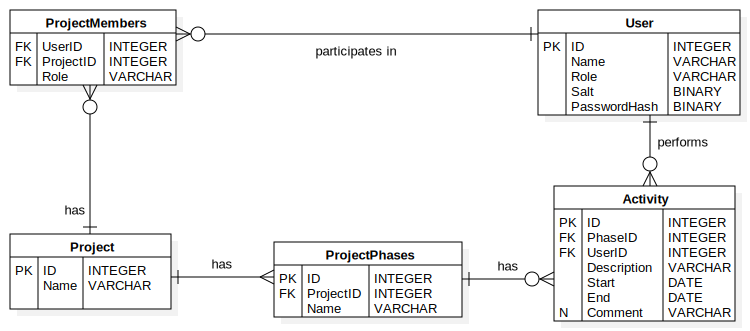
\includegraphics[width=\textwidth]{./content/pictures/database.png}
\caption{Database diagram}
\label{fig:database}
\end{figure}

\clearpage

\section{Phase 1: One Databse and UI}
\subsection{Monolithic Code Samples}
%\subsubsection{Database Access}
%\subsubsection{UI Interaction}

\subsection{Best-Practice Code Samples}
%\subsubsection{Database Access}
%\subsubsection{UI Interaction}

\section{Phase 2: More Databases / UIs}

\subsection{Monolithic Code Samples}
%\subsubsection{Database Access}
%\subsubsection{UI Interaction}

\subsection{Best-Practice Code Samples}
%\subsubsection{Database Access}
%\subsubsection{UI Interaction}
\chapter{Results}

\section{Lines of Code}
\section{Programming Effort}
\section{Efficiency and Performance}
\section{Touched and Edited Files}
\section{Readability}
\chapter{Discussion}
\label{sec:discussion}
In this chapter all data gathered in the last section is revisited and put into context. 
\section{Meaning and significance of the file count}
As clearly visible in section \ref{sec:file-count} the ad-hoc version of the program does not need as many files as the best practice implementation. This is mainly due to the missing interface files, as well as the files for repositories. Especially in phase 3, where a new database should be supported, this factor can be easily observed. In the ad-hoc version all code concerning the database interaction was put into existing classes, resulting in only one additional file while the best practice implementation needs to create and derive one file per repository. 

\section{Meaning and significance of the line count}
The same statement as above applies to the count of total lines as seen in section \ref{sec:line-count}. Each interface class consists of various method declarations that are counted as well. As stated in the footnote of table \ref{table:lines-of-code} for better comparison in addition to the total line count for the best practice implementation another count was made excluding the \texttt{@Override}-Annotation lines as they bias the result. 

Here a interesting observation can be made for the line count: While the total count of the best practice version is higher for both phases 1 and two, the increase of lines is between the phases is significantly lower. While the best practice version added 2960 lines of code, the ad-hoc version added 3600 lines of code. This difference of about 700 lines does not seem much, however it has to be noted that this lines were mainly necessary because of case distinctions as can be seen in section \ref{sec:ad-hoc-javafx}. This reduces readability on the one hand and results in a greater risk of programming errors. 

The fact that the increase in lines between phase 2 and 3 is nearly the same is easily explained as the added files differ significantly. Due to the overhead of declaring a class including its constructor etcetera leads to a high number of additions which are not necessary in the ad-hoc version.

Consequentially to the lower number of files and the comparable number of lines in the two programs, the ad-hoc implementation on average contains noticeably more code per file. As the two implementations offer exact the same functionality this means that responsibilities have shifted and each class is in charge of more actions. However this fact is a clear violation of the Single-Responsibility-Principle (see section \ref{sec:srp}) which may introduce more programming errors in the future. 

\section{Maintainability}
The biggest effect and difference when using design patterns and interfaces can be observed exactly in conforming of the Single-Responsibility-Principle and hence in the readability of the code. While each data class of the ad-hoc version does not only have the responsibility to encapsulate the data, it is responsible for saving the data to two different kinds of persistent storage. This results in a quite long file that mixes technologies and needs to be revisited any time a new persistent storage is added, existing storage technologies are changed or the data classes change. 

In the case of view frameworks due to missing use of interfaces asides from implementing the view using a new framework each and every class that depends on any kind of interface needs to be adopted. This is visible in table \ref{table:touched-files}, where is stated that the implementation of new technologies influences lower numbers of dependent files which is a very desired behaviour. 
\chapter{Conclusion}

In the last chapters some interesting findings were gathered. Two program versions were compared, one following best practice guidelines in the sense of object oriented programming, the other one featured ad-hoc programming without paying attention to topics of software maintenance.

Throughout the development process six major issues could be discovered:

\begin{itemize}
	\item \textbf{Number of files}: The best practice version of the application needed a higher number of files than the ad-hoc implementation throughout all phases.
	\item \textbf{Lines of code}: The best practice version needed more lines of code in all phases.
	\item \textbf{Lines per file}: The best practice versions files contained notably less lines of code per file.
	\item \textbf{Increase in code lines}: Especially in transition from phase 1 to phase 2 the best practice implementation needed considerably less code additions.
	\item \textbf{Touched files}: The number of touched or edited files during phase transition was lower in the best practice program version.
	\item \textbf{Code Complexity}: The ad-hoc implementations code complexity increases more rapidly during the phase transitions and lays considerably above the complexity of the best practice program version.
\end{itemize}

It has to be said that the results gathered in section \ref{sec:results} may vary depending on the coding style, programming language, concrete use case and size of the project, furthermore the term \emph{code quality} does not have a unique definition. There are many different standpoints on what attributes a well written code should have, often depending on company coding policies. One factor that is not mentioned by intention in this thesis is the readability of the code as this is a very subjective matter and is therefore not considered. 

In terms of the definition used in this thesis, which mainly focuses on properties defined by guidelines of the object oriented programming the results support the hypothesis saying that the use of design patterns improves code quality in later stages of a project cycle. This is backed up by the lower number of files needing modification in the process of extending functionality and the lower number of lines added between phases 1 and 2 as well as the increase in code complexity between those two phases.

At the same time in the first stage the initial programming effort for a clean implementation using well-known patterns is considerably higher, and even later on in the best practice implementation utilizes both a larger number of files and more lines of code, which may increase the efforts for software maintenance and testing.

In conclusion it can be said that the use of design patterns can help to increase code quality if the requirements of a software project are likely to change, which is the common case especially for bigger applications. 

As this work only focuses on a small number of design patterns and other literature does not come to clear results as well, further research is certainly necessary. If future work is focusing on existing software projects, challenges will likely include the difficulties in comparing different approaches applied in the compared applications. However if new research rather studies effects of design patterns by observing controlled experiments, as this thesis does, the main challenge will likely include the question if small scale results also apply for enterprise scale applications.


%\chapter{Future Work}
\section{Physical Seperation of Tiers}


%\cite{Gof94}
%\cite{Hfd04}
%\cite{Aspect06}
%\cite{Composing06}

\cleardoublepage

\let\LaTeXStandardClearpage\clearpage
\let\clearpage\relax  % Do nothing when a \clearpage command appears 
\let\cleardoublepage\relax
\printbibliography	
\listoffigures
\listoftables
\lstlistoflistings

\let\clearpage\LaTeXStandardClearpage % Return to the old definition

\end{document}

